% Task 2: RC4 as a black box. Values from Task2/use_rc4.py and Task2/rc4.py;
% CHECKED (python3): keystream(b"Kangaroo", 8) = 69 9d da 7e fe 61 73 62;
%   the ciphertext starts 24 F8 BF 0A DE 0C 16 42 and has 28 bytes.
%   The plaintext and the keystream of "Kangarop" are the results of the task: not shown.
\documentclass[12pt,tikz,border=6pt]{standalone}
% Shared preamble of the task figures of Lecture 1.
% The colours and styles are copied from the preamble of ../main.tex (keep them in sync).
\usepackage{lmodern}
\usepackage[T1]{fontenc}
\renewcommand{\familydefault}{\sfdefault}
\usepackage{amsmath,amssymb}
\usepackage{xcolor}
\usepackage{fontawesome5}
\usetikzlibrary{arrows.meta, calc, positioning, fit, decorations.pathreplacing, decorations.pathmorphing, backgrounds}

% ---------- template ----------
\definecolor{DeepBlue}{HTML}{283593}
\definecolor{AccentOrange}{HTML}{EB5A14}
\definecolor{LightGray}{HTML}{F5F6FA}
% ---------- actors and categories (S1 to S6) ----------
\definecolor{sIndigo}{HTML}{5C6BC0}   % the sender
\definecolor{sPink}{HTML}{EC407A}     % the attacker
\definecolor{sViolet}{HTML}{7E57C2}   % plaintext
\definecolor{sAmber}{HTML}{FFB300}    % key and keystream
\definecolor{sTeal}{HTML}{26A69A}     % the receiver
\definecolor{sBrown}{HTML}{8D6E63}    % ciphertext
\definecolor{sPinkText}{HTML}{C2185B}
\definecolor{sAmberText}{HTML}{A06A00}
\definecolor{sTealText}{HTML}{00796B}
% ---------- actions and results ----------
\definecolor{aExec}{HTML}{43A047}
\definecolor{aRead}{HTML}{1E88E5}
\definecolor{aWrite}{HTML}{E53935}
% ---------- neutral ----------
\definecolor{nInk}{HTML}{37474F}
\definecolor{nLine}{HTML}{90A4AE}
\definecolor{nLight}{HTML}{CFD8DC}
\definecolor{nFill}{HTML}{ECEFF1}
\definecolor{nIdle}{HTML}{E0E0E0}

% ---------- TikZ styles (as in main.tex; byte cells a little larger for the web) ----------
\tikzset{
  hw/.style={draw=nLine, thick, fill=nFill, text=nInk, rounded corners=3pt, align=center, inner sep=4pt},
  hwmain/.style={draw=nInk, thick, fill=nInk, text=white, rounded corners=3pt, align=center, inner sep=4pt},
  cell/.style={draw=nLine, thick, fill=white, text=nInk, font=\ttfamily\small},
  cellfree/.style={cell, dashed, draw=nLight},
  container/.style={draw=nLine, thick, dashed, rounded corners=5pt},
  actor/.style={fill=#1, draw=#1, text=white, rounded corners=3pt, align=center, font=\small\bfseries, inner sep=5pt},
  actorlight/.style={fill=#1!15, draw=#1, thick, text=nInk, rounded corners=3pt, align=center, inner sep=5pt},
  data/.style={-{Stealth}, very thick, nInk},
  flow/.style={-{Stealth}, very thick, DeepBlue},
  annot/.style={draw=AccentOrange, line width=1.6pt, rounded corners=3pt},
  byte/.style={draw=nLine, thick, fill=white, text=nInk, font=\ttfamily\small,
    minimum width=0.8cm, minimum height=0.62cm, inner sep=1pt, rounded corners=1.5pt},
  ptb/.style={byte, fill=sViolet!15, draw=sViolet},
  ksb/.style={byte, fill=sAmber!25, draw=sAmber},
  ctb/.style={byte, fill=sBrown!15, draw=sBrown},
  unk/.style={byte, fill=white, dashed, text=sViolet},
  rowlabel/.style={font=\small\bfseries, text=nInk, anchor=east},
  note/.style={font=\small, text=nInk},
  bigxor/.style={circle, draw=nInk, very thick, fill=white, inner sep=0pt, minimum size=0.8cm, font=\Large},
  radio/.style={-{Stealth}, very thick, nInk, decorate,
    decoration={snake, amplitude=1.2pt, segment length=7pt, post length=4pt}},
  % a white card behind the whole figure, so that it stays readable in a dark theme
  card/.style={show background rectangle, background rectangle/.style={fill=white, draw=none}, inner frame sep=8pt},
}
% a row of bytes: \byterow{x of the first cell}{y}{style}{list of values}{step between cells}
\newcommand{\byterow}[5]{%
  \expandafter\def\expandafter\brlist\expandafter{#4}%
  \foreach \v [count=\k from 0] in \brlist {
    \node[#3] at ({#1+#5*\k},#2) {\v};
  }}
% the generator / cipher box: dark, with cogs. \cogbox{name}{position}{label}{width}
\newcommand{\cogbox}[4]{%
  \node[hwmain, minimum width=#4, minimum height=1.3cm] (#1) at (#2) {};
  \node[text=white, font=\Large] at ([yshift=0.22cm]#1.center) {\faCogs};
  \node[text=white, font=\small\bfseries] at ([yshift=-0.32cm]#1.center) {#3};}
\newcommand{\ok}{\textcolor{aExec}{\faCheck}}
\newcommand{\nok}{\textcolor{aWrite}{\faTimes}}
\newcommand{\badge}[1]{\tikz[baseline=(b.base)]\node[circle,fill=AccentOrange,text=white,
  inner sep=1.5pt,font=\bfseries\footnotesize] (b) {#1};}

\begin{document}
\pagecolor{white}
\begin{tikzpicture}[>=Stealth]
  \def\dx{1.0}
  \def\xs{7.0}
  % key -> RC4 -> keystream
  \node[actorlight=sAmber, font=\small, minimum height=1.0cm, align=center] (k) at (0,0)
    {\faKey\ \textbf{key}\\ \texttt{b"Kangaroo"}};
  \node[hwmain, minimum width=2.6cm, minimum height=1.3cm] (r) at (3.5,0) {};
  \node[text=white, font=\Large] at (2.85,0.18) {\faCogs};
  \node[text=white, font=\large\bfseries] at (3.85,0.18) {RC4};
  \node[text=white, font=\scriptsize] at (3.5,-0.35) {black box};
  \draw[data] (k) -- (r);
  \draw[data] (r.east) -- (6.45,0);
  \node[font=\ttfamily\small, text=nInk, anchor=south] at (3.5,0.75) {keystream(key, 28)};
  \byterow{\xs}{0}{ksb}{69,9D,DA,7E,FE,61,73,62}{\dx}
  \node[font=\large, text=nInk] at ({\xs+8*\dx},0) {\ldots};
  \draw[decorate, decoration={brace, amplitude=5pt}, nInk] ({\xs-0.4},0.45) -- ({\xs+8.3*\dx},0.45)
    node[midway, above=6pt, note] {\textbf{keystream}: 28 bytes, as long as the ciphertext};
  % XOR with the ciphertext
  \node[rowlabel] at ({\xs-0.55},-1.25) {ciphertext};
  \byterow{\xs}{-1.25}{ctb}{24,F8,BF,0A,DE,0C,16,42}{\dx}
  \node[font=\large, text=nInk] at ({\xs+8*\dx},-1.25) {\ldots};
  \node[font=\small\bfseries, text=nInk, anchor=east] at ({\xs-0.55},-0.62) {XOR};
  \draw[nInk, thick] ({\xs-0.45},-1.78) -- ({\xs+8.3*\dx},-1.78);
  \node[rowlabel] at ({\xs-0.55},-2.3) {message};
  \foreach \k in {0,...,7} \node[unk] at ({\xs+\dx*\k},-2.3) {?};
  \node[font=\large, text=nInk] at ({\xs+8*\dx},-2.3) {\ldots};
  \node[font=\small, text=AccentOrange, anchor=west] at ({\xs+8.5*\dx},-2.3) {\badge{2}};
  \node[font=\small, text=AccentOrange, anchor=west] at ({\xs+8.5*\dx},0) {\badge{1}};

  % one letter of the key changed
  \draw[nLight, thick, dashed] (-1.4,-3.05) -- (17.0,-3.05);
  \node[actorlight=sAmber, font=\small, minimum height=1.0cm, align=center] (k2) at (0,-4.5)
    {\faKey\ \textbf{key}\\ \texttt{b"Kangaro\textcolor{AccentOrange}{\textbf{p}}"}};
  \node[hwmain, minimum width=2.6cm, minimum height=1.3cm] (r2) at (3.5,-4.5) {};
  \node[text=white, font=\Large] at (2.85,-4.32) {\faCogs};
  \node[text=white, font=\large\bfseries] at (3.85,-4.32) {RC4};
  \node[text=white, font=\scriptsize] at (3.5,-4.85) {black box};
  \draw[data] (k2) -- (r2);
  \draw[data] (r2.east) -- (6.45,-4.5);
  \node[font=\ttfamily\small, text=nInk, anchor=south] at (3.5,-3.75) {keystream(b"Kangarop", 8)};
  \foreach \k in {0,...,7} \node[byte, fill=white, dashed, draw=sAmber, text=sAmberText] at ({\xs+\dx*\k},-4.5) {?};
  \node[font=\small, text=AccentOrange, anchor=west] at ({\xs+8.5*\dx},-4.5) {\badge{3}};
  \node[note, anchor=north, align=center] at ({\xs+3.5*\dx},-5.0)
    {only the last letter changed: \textbf{how many of the 8 bytes stay the same?}};
\end{tikzpicture}
\end{document}
